
%quantitative-fvr experiments
%stereo-
%fvr-sota
%mvvdscfds%%%r
%qual
%

In order to quantitatively compare and analyse the FVR, FFVR, FVR-3D and MVVR extensions, several real world data sets were captured using: stereo camera, active camera and monocular camera set-ups. In the case of Stereo sensor input, several City scenes from the Kitti Vision Benchmark Data Set were chosen. These scenes contain accurate laser scans, stereo gray-scale images, stereo rgb-images and GPS and IMU data. In order to simulate the theoretical situation in which stereo cameras generate the most accurate depth maps, the laser scans are used in place of depth data computed by a disparity algorithm. Therefore in our experiments on these stereo data, only the laser scans and stereo gray-scale images are used. \\

The 5 stereo data-sets used in the experiments are shown in appendix \ref{StereoSensorDataSet}. The first scene is the Kitti 0001 Sync Data Set, this scene has 114 frames. This data set contains 12 cars, 2 cyclists and a tram. The tram and cyclists are non static objects within the scene, making it more difficult for the current set of reconstruction algorithms which rely on scenes being primarily static in nature. To the right in this dataset, there is a tram-line and some trees and gardens, to the left is a residential street. The second scene is the Kitti 0002 Sync Data Set, this set is 83 frames long. It contains 1 car and two cyclists which are non-static objects. Within this scene there is a long brick wall hiding some tall trees, several cyclists ride along next to the wall. To the left, there are are some grassy areas, some buildings and some parked cars. \\

At 160 frames, the Kitti 0005 Sync Data Set is also used. This scene contains 9 cars, 3 vans, 2 pedestrians and 1 cyclist. Because of the size of the van and the other non-static objects within the scene, this appears to be one of the more difficult scenes to register. The camera winds through several different streets as opposed to the previous data sets which are mostly of one long road. The fourth dataset used, the Kitti 0091 Sync Data Set is composed of 346 frames making it the largest data set used in these experiments. This data set contains 2 cars, a van, 42 pedestrians, 14 sitters, 8 cyclists and 1 miscellaneous object. Due to containing so many non-static objects this scene is also considered difficult like the Kitti 0005 Data Set. \\

The last Kitti Vision Benchmark Data Set used is the Kitti 0095 Data Set. Unlike the previous data sets, all 274 frames only contain static object, and the scenes are made up primarily of small winding streets. \\ 

In order to assess results using an active camera sensor, test data was generated using the ASUS Xtion PRO LIVE camera. Because these data sets were generated during experimentation, the opportunity was taken to generate scenes, each captured using a specific type of camera movement. Some scenes were captured by rotating the camera about the x or y-axes, others by translating the camera. By testing with different movements, future algorithms may be constructed by switching to different registration methods based on camera movement. The different camera transformations recorded in the test data include: translation (left and right), and rotation about different axes (x and y axis). \\

Some samples from these data sets are shown in appendix \ref{ActiveSensorDataSet}. The first scene: the Apartment Texture Rotate scene was taken by rotating the camera around the y-axis across an apartment. This scene contains a lot of texture information. The Apartment Texture X Axis scene is similar in terms of texture but contains both x and y axis rotation. This tests the FVR's ability to handle multiple axes of rotation. The Office textured blind-spot rotation scene is a textured office scene where the camera is rotated about the y-axis. The scene is focused on a large divider which separates two desks. The divider may confuse registration methods which rely too heavily on minimization by aligning the large divider as a priority rather than taking into account the smaller details within the scene. An example of such an algorithm would be ICP and its derivatives. The Office scenes contain a plenty of usable texture and different sets were created by translating, rotating about the y-axis and rotating about the x-axis. \\


The MVVR method was analysed using test data generated using a Microsoft passive RGB camera or the rgb component of the ASUS Xtion PRO LIVE active camera. The data output is in basic video format, and all depth information was generated implicitly by the MVVR algorithm. This data was captured by moving the camera whilst focusing on a set of textured boxes within an indoor environment. Several frames were captured at 30 frames per second and registered for analysis of the MVVR method qualitatively. Quantitative tests of the MVVR make use of the same data as tests for the FVR method (testing translation and rotational registration error). \\

To assess qualitative reconstruction, three scenes were captured and registered using the FVR method. These scenes include the apartment scene, office scene and the garden scene. All three scenes were captured using the Asus XTION PRO live active camera at 30 frames per second. For each scene, only one in every 30 frames were registered, constituting real time FVR performance. The apartment scene was generated by moving and rotating the camera around an apartment living room before moving towards the kitchen area. This scene contains an abundance of features and would be considered a basic test for most 3D reconstruction algorithms. The second scene is the Office scene. This scene was generated by rotating the camera whilst zooming in and out on different objects within the room. Again this scene was reconstructed by registering every 30th frame. Despite both of the scenes being trivial to reconstruct, most algorithms (especially feature matching based methods) would find registering large rotations (such as those present in this data) difficult. The Garden scene is a difficult scene to reconstruct regardless of the reconstruction algorithm or technique used for registration. This scene was captured by rotating the camera around a garden outside the university. The scene contains many textures which are similar at the local level but are located in totally different locations. Therefore the scene is difficult to reconstruct using local and feature based methods such as FM+RANSAC and ICP. \\


\begin{figure}[!htb]
\centering
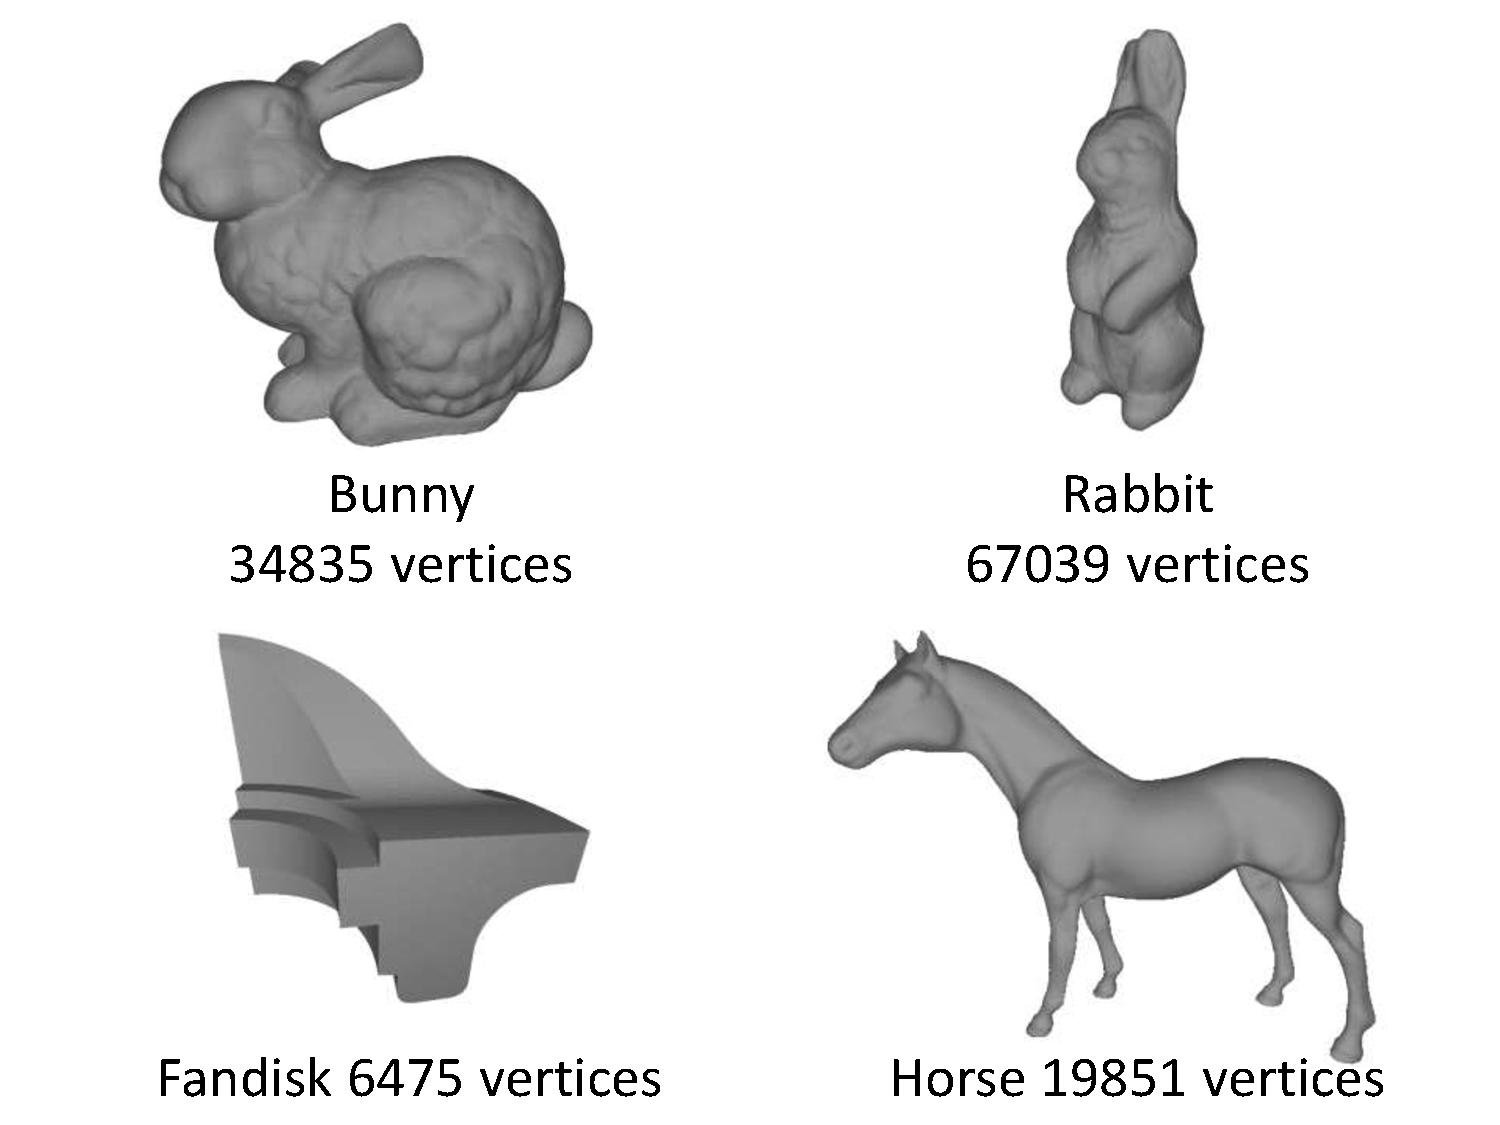
\includegraphics[width=4.0in]{images/experiments/test_data/modelsused}
\caption{Models used to assess the Plane-Tree compression algorithm.}
\label{fig:MODELSUSEDA}
\end{figure}

To test the Plane-Tree algorithm, several 3D objects commonly used within the literature were used to compare with known state of the art compression methods in terms of 3D mesh compression. The models used for testing are shown in figure \ref{fig:MODELSUSEDA}. These include: the bunny model with 34835 vertices, the rabbit model with 67039 vertices, the fandisk model with 6475 vertices and the horse model with 19851 vertices. \\

Several 3D reconstructions generated from the data set in appendix \ref{AppendixA} were used also to assess the Plane-Tree in compressing 3D reconstructions for storage and transmission. \\

